\section{Evaluation} \label{sec:evaluation}

In order to evaluate the impact of migrating a process with an established TCP connection, we are interested in assessing how quickly can communication resume after restore.

To achieve this goal we set up the following testbed.
We first deploy two identical virtual machines running Linux Debian with kernel version \texttt{4.19.0-6}.
Each one has \criu version 3.13 and \runc version \texttt{1.0.0-rc8}, both built from source.
Additionally, and in order to conduct the experiments, we make use of \texttt{iPerf3} (version \texttt{3.7+}) a network bandwidth benchmarking tool~\cite{iperf3}.
In particular, we start an \texttt{iPerf3} client-server pair, one in each VM, and record the perceived throughput by the client.
Each experiment is repeated running the bare processes and checkpointing them using \criu, or isolating them within a \runc container, to assess the introduced overhead.
We measure from the client side since we are interested in dumping and restoring the server.
This situation makes more sense from the cloud-provider/load-balancing standpoint.

\textbf{Re-connection after a down period.}
The first experiment simulates the scenario in which the server is restored some time after the dump occured.
In particular, we let the client saturate the link for 10 seconds, then dump the server, and restore it 2 seconds later, all of which transparently to the client (whose connection is never closed).
In Figure~\ref{fig:evaluation-downtime} we present the throughput perceived by the client as a function of time. 
\begin{figure}[h!]
    \centering
    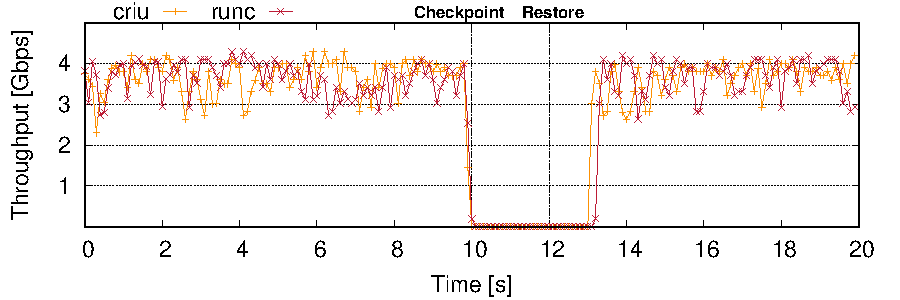
\includegraphics[width=\linewidth]{./images/tcp_established_downtime_microbenchmark.pdf}
    \caption{Throughput perceived from the client as a function of time, when we checkpoint the server once, and restore it after two seconds. We compare the results of \criu and \runc. \label{fig:evaluation-downtime}}
\end{figure}
The first observation we make from the plot, is that it takes almost a full second to get the connection back to full speed.
To understand this behaviour we must recall what is \texttt{iPerf3} actually doing.
The client tries to saturate the link, sending as many packets as it can, and reports the measured capacity.
As the socket is never closed, and packets are just discarded by the network filters, to the client it will be as if those packets were never acknowledged, and hence will try to retransmit them.
The TCP protocol specifies~\cite{tcp-rfc} that the retransmission timeout must be doubled every time a packet is not acknowledged, therefore the recurrent outage of ACKs might cause the client to back-off for the perceived full second.
This implies that checkpointing established TCP connections only makes sense in the scenario in which the service is soon going to be restored.
The next experiment tackles the behaviour under this situation.

\textbf{Reactivity to immediate restore.}
To prove our hypothesis that the large delay after a restore is due to the protocol itself rather than our implementation, we set up an experiment in which we perform a sequence of dumps and immediate restores of the same established TCP connection.
We again present the throughput as a function of time in Figure~\ref{fig:evaluation-reactivity}.
\begin{figure}[h!]
    \centering
    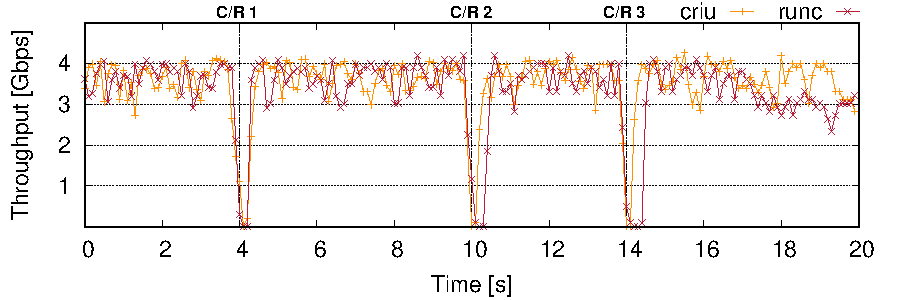
\includegraphics[width=\linewidth]{./images/tcp_established_resolution_microbenchmark.pdf}
    \caption{Throughput from the client as a function of time.\label{fig:evaluation-reactivity}}
\end{figure}
In this case the measured throughput downtime does not exceed $0.1$ seconds, an order of magnitude better than the previous experiment.
This reduced value, together with the fact that the application studied is very network-intensive, makes us believe that our proposed technique is suitable for most client-server scenarios and won't have an impact in the overall quality of service.

Lastly, in both Figures we observe that, albeit being the experiments running bare processes with \criu slightly faster to restore, the overhead introduced by \runc is negligible.
